%! Author = drakanoy
%! Date = 10.09.2024

% Preamble
\documentclass[12pt]{article}

% Packages
\usepackage[utf8]{inputenc}
\usepackage[T2A]{fontenc}
\usepackage[english, russian]{babel}
\usepackage[a4paper, includefoot, left=1.5cm, right=1.5cm, top=1cm, bottom=1.5cm, headsep=1cm, footskip=1cm]{geometry}
\usepackage{makecell}
\usepackage{amsmath}
\usepackage{graphicx}
\usepackage{enumitem}
\usepackage{svg}
\usepackage{multirow}
\usepackage{hyperref}
\usepackage{mathtools}
\usepackage{amssymb}
\usepackage{textcomp}

% Document
\begin{document}
\begin{large}
\begin{center}
\LARGE \textbf{Домашняя работа}
\par
\LARGE \textbf{Кононов Александр Михайлович}
\par
    \textbf{9.11.2024}
\end{center}
\par Условие:
\par
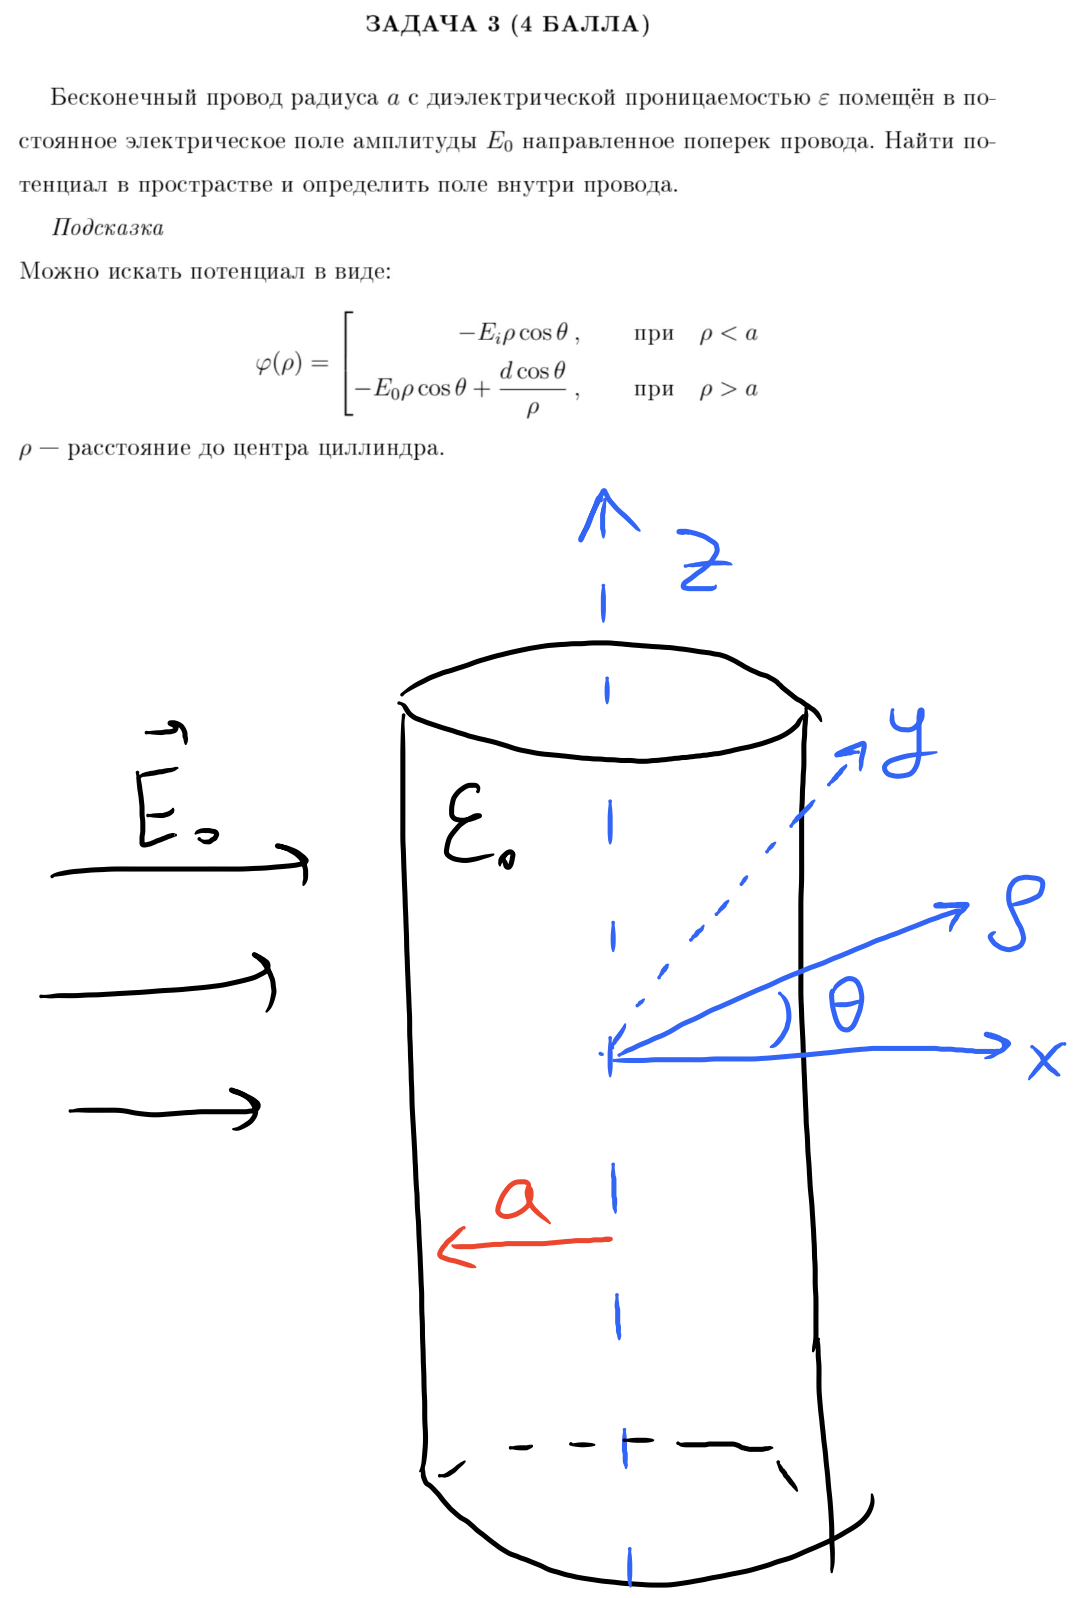
\includegraphics[width=1\textwidth]{photo.png}
%\begin{center}
%\underline{Рисунок 1}:
%\end{center}
\par Решение:
\par
\par
%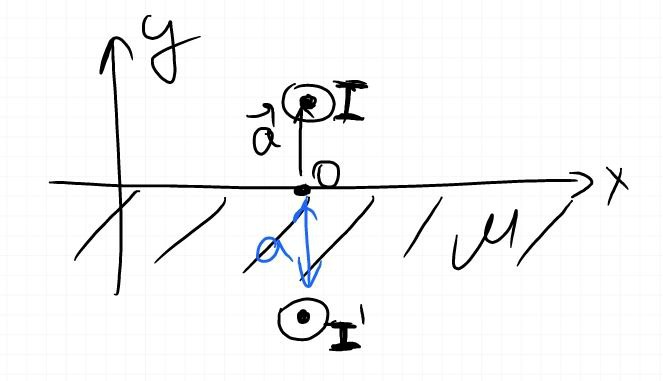
\includegraphics[width=1\textwidth]{photo_1.jpg}
%\par
%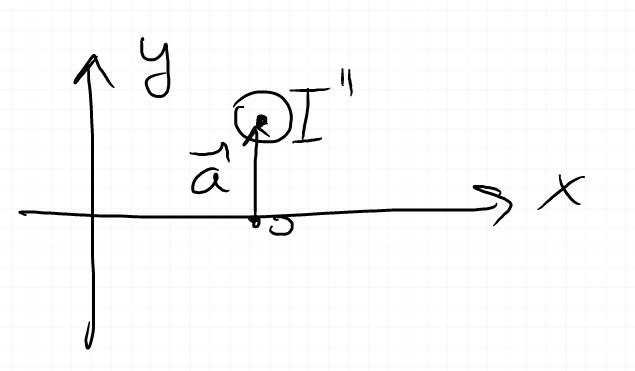
\includegraphics[width=1\textwidth]{photo_2.jpg}
\par
\[
    \frac{n_x^2}{\varepsilon_{\parallel}} + \frac{n_z^2}{\varepsilon_{\perp}} = 1
\]
\[
    n_z = \sqrt{\varepsilon_{\perp} - \frac{\varepsilon_{\perp}}{\varepsilon_{\parallel}} n_x^2 }
\]
\par В вакууме: $n_x = \sin \theta$, при переходе в кристалл эта компонента сохраняется
\[
    n_z = \sqrt{\varepsilon_{\perp} - \frac{\varepsilon_{\perp}}{\varepsilon_{\parallel}} \sin^2 \theta}
\]
\par Отношение компонент лучевых скоростей:
\[
    tg \theta' = \frac{s_x'}{s_z'} = \frac{\varepsilon_{\perp} n_x}{\varepsilon_{\parallel} n_z} = \frac{\varepsilon_{\perp} \sin \theta}{\varepsilon_{\parallel} \sqrt{\varepsilon_{\perp} - \frac{\varepsilon_{\perp}}{\varepsilon_{\parallel}} \sin^2 \theta}}
\]
\par Ответ:

\[
    tg \theta' = \frac{s_x'}{s_z'} = \frac{\varepsilon_{\perp} n_x}{\varepsilon_{\parallel} n_z} = \frac{\varepsilon_{\perp} \sin \theta}{\varepsilon_{\parallel} \sqrt{\varepsilon_{\perp} - \frac{\varepsilon_{\perp}}{\varepsilon_{\parallel}} \sin^2 \theta}}
\]

\end{large}
\end{document}
